\documentclass{article}

\usepackage{amsmath}
\usepackage{fancyhdr}
\usepackage{graphicx}
\graphicspath{{}}

%% some colours
\usepackage{color}
\definecolor{deepblue}{rgb}{0,0,0.5}
\definecolor{deepred}{rgb}{0.6,0,0}
\definecolor{deepgreen}{rgb}{0,0.5,0}
\definecolor{backcolour}{rgb}{0.95,0.96,0.93}

%%%%%%%%%%%%%% CODE STUFF %%%%%%%%%%%%%%
%%%%%%%%%%%%%%%%%%%%%%%%%%%%%%%%%%%%%%%%
\usepackage{cprotect} % to be used in sol
\usepackage{listings} % for code display
% setting code style
\newcommand\pythonstyle{\lstset{
        language=Python,
        backgroundcolor=\color{backcolour},
		basicstyle=\footnotesize,
		otherkeywords={self},
		keywordstyle=\footnotesize\color{deepblue},
		emph={__init__},
		emphstyle=\footnotesize\color{deepred},
		stringstyle=\color{deepgreen},
		frame=single,
		showstringspaces=false  ,
		breaklines=true,
		numbers=left,
		numberstyle=\footnotesize,
		tabsize=4,
		breakatwhitespace=false
	}}

% Python environment
\lstnewenvironment{python}[1][]{
    \pythonstyle
    \lstset{#1}
}{}

% Python for external files
\newcommand\pythonexternal[2][]{{
    \pythonstyle
    \lstinputlisting[#1]{#2}
}}

% Python for inline
\newcommand\pythoninline[1]{{\pythonstyle\lstinline!#1!}}

%%%%%%%%%%%%%%%%%%%%%%%%%%%%%%%%%%%%%%%%
% setting the style for ex documents
\pagestyle{fancy}
\fancyhf{}
\fancyhead[L]{\thetitle}
\fancyhead[C]{}
\fancyhead[R]{\theauthor}
\renewcommand{\headrulewidth}{0.4pt} %obere Trennlinie
\fancyfoot[L]{Due: \thedate}
\fancyfoot[R]{\thepage} %Seitennummer
\renewcommand{\footrulewidth}{0.4pt}

% include solutions
\newcommand\sol[1]{{\large\textbf{\\Solution:}}#1}
\usepackage{tikz}
\usetikzlibrary{arrows,automata}

\title{BPP Exercise 6 - Sorting and IO}
\author{A. Hain, M. Nipshagen}
\date{14.05.2018, 08:00}

\makeatletter
\let\thetitle\@title
\let\theauthor\@author
\let\thedate\@date
\makeatother

% do not include solutions
% \renewcommand\sol[1]{}


\begin{document}

The deadline for this exercise sheet is \textbf{Monday, \thedate.}
%
%\section*{Introductory Words}
%In case we have some information that doesn't directly concern the current exercises.
%

\section{Warm-Up}

\subsection{Key Sort}
Given a list of the following structure:
\begin{python}
my_lst = [
  {
    "key1" : value1,
    "key2" : value2,
    "key3" : value3
  },
  {
    "key1" : a_value,
    "key2" : b_value,
    "key3" : c_value
  },
  ...
]
\end{python}
Sort the list in such a way, that the value of \texttt{"key2"} is used to compare and sort the dictionaries inside the list. In the file 
\texttt{task\_1.py} you can find an example dictionary as well as a sorted
version to compare to when you are done.
\\
\cprotect\sol{
\begin{python}
sorted(my_lst, key=lambda x: x["key2"])
\end{python}
}

\subsection{Read \& Write}
In the file \texttt{task\_1.txt}, is an unsorted list of numbers. Read in the list, sort it in \textit{descending} order and write it back to the file.
In the end the file should only contain the sorted list.\\
\cprotect\sol{
\begin{python}
with open("./task_1.txt", "r+") as f:
    lst_in = f.read() # read the list as string
    lst_in = lst_in[1:-1] # get rid of the brackets
    # split on the commas of the list,
    # and cast to float since we are dealing with numbers
    lst = [float(x) for x in lst_in.split(",")]
    lst.sort(reverse=True) # and sort
    f.write(str(lst)) # back in the file it goes
\end{python}
}

\section{Powering through I/O}
Let's make a game! In Hangman, one player -- in our case this will be the
computer -- picks a random word and tells the other player(s) how many
letters it has -- usually displayed through underscores. For example, if
the word is \texttt{hello} we would get \verb|_ _ _ _ _|.\\
The other player(s) now have to guess the word letter by letter. If a
letter that is part of the word is guessed, it is revealed. To
continue our example, if you would guess an \textbf{e} the computer would
reveal it and the new game state would be \verb|_ e _ _ _|. If your next
guess would be an \textbf{l} the new game state would be \verb|_ e l l _|.
If you guessed the whole word, you win the game!\\
But there is a catch: Traditionally, at the start of the game you would
draw empty gallows, and every time you guessed a letter that is
\textit{not} in the word, you would draw one more part of a man hanging --
thus the name hangman (see \ref{fig:hangman}). If you guess the word
before the man is complete, you win! Otherwise the stick figure has 
come to a tragic end and you lose.\\
Since it might be hard to visualise the hangman on the terminal (you are 
very welcome to try it out though), you might want to use just a counter.

\subsection*{Task}
Write a \texttt{hangman.py} script which implements a version of the 
hangman game. In the supplied \textbf{.zip} file you can find a 
\texttt{words.txt}, which you should use to read in the list of possible
words. You are welcome to change the file though.\\
An example pseudocode:
\begin{verbatim}
Set number of misses
Read in possible words
Choose a word
Prepare guessword with underscores
Display the rule set
While not guessed and more than 0 misses left:
  Display current game state
  Get a guess letter as user input
  If guessed letter is in the word:
    Update the guess word
    If guessed:
      win
  Else:
    Update list of failes and misses
    If no misses left:
      Lose
\end{verbatim}

\subsection*{Hints}
\begin{itemize}
  \item Remember that strings are immutable, so you can not do:
\begin{python}
a = 'hello'
a[3] = 'a
\end{python}
  \item You can instead display the guessword as a list of underscores
\begin{python}
word = 'hello'
guess_word = ['_', '_', '_', '_', '_']
\end{python}
  \item Whenever you have gotten an input letter, check whether it is
  part of the word. You can use the \pythoninline{in} keyword and the
  \pythoninline{word.index(input_char)} function for this.
\begin{python}
if 'l' in word:
  guess_word[word.index('l')] = 'l'
\end{python}
\emph{Note:} This code snippet probably is not how you are going to
use it. But it might point you in the right direction.
  \item Similarly, you can use \texttt{in} to check whether the player
  has won.
  \item For choosing a word, you could take a look at the \texttt{choice}
  function from the \texttt{random} module. You can read upon it here:
  \url{https://docs.python.org/3.5/library/random.html#random.choice}.\\
  And you can use it with the following structure:
\begin{python}
import random


random.choise(my_list)
\end{python}
\end{itemize}
It might be a good idea to split your code into several smaller functions,
which each perform a single task. For example, one function which checks
whether the player has won, one function to print the current game state,
one to read in the file, and one to pick a word, and so on. Then combine
those functions to build your whole game.\\
Please note, that the hints are just that: hints for a possible solution
to a problem. Your program can be perfectly fine without using any of
the hints.


\begin{figure}[ht]
\centering
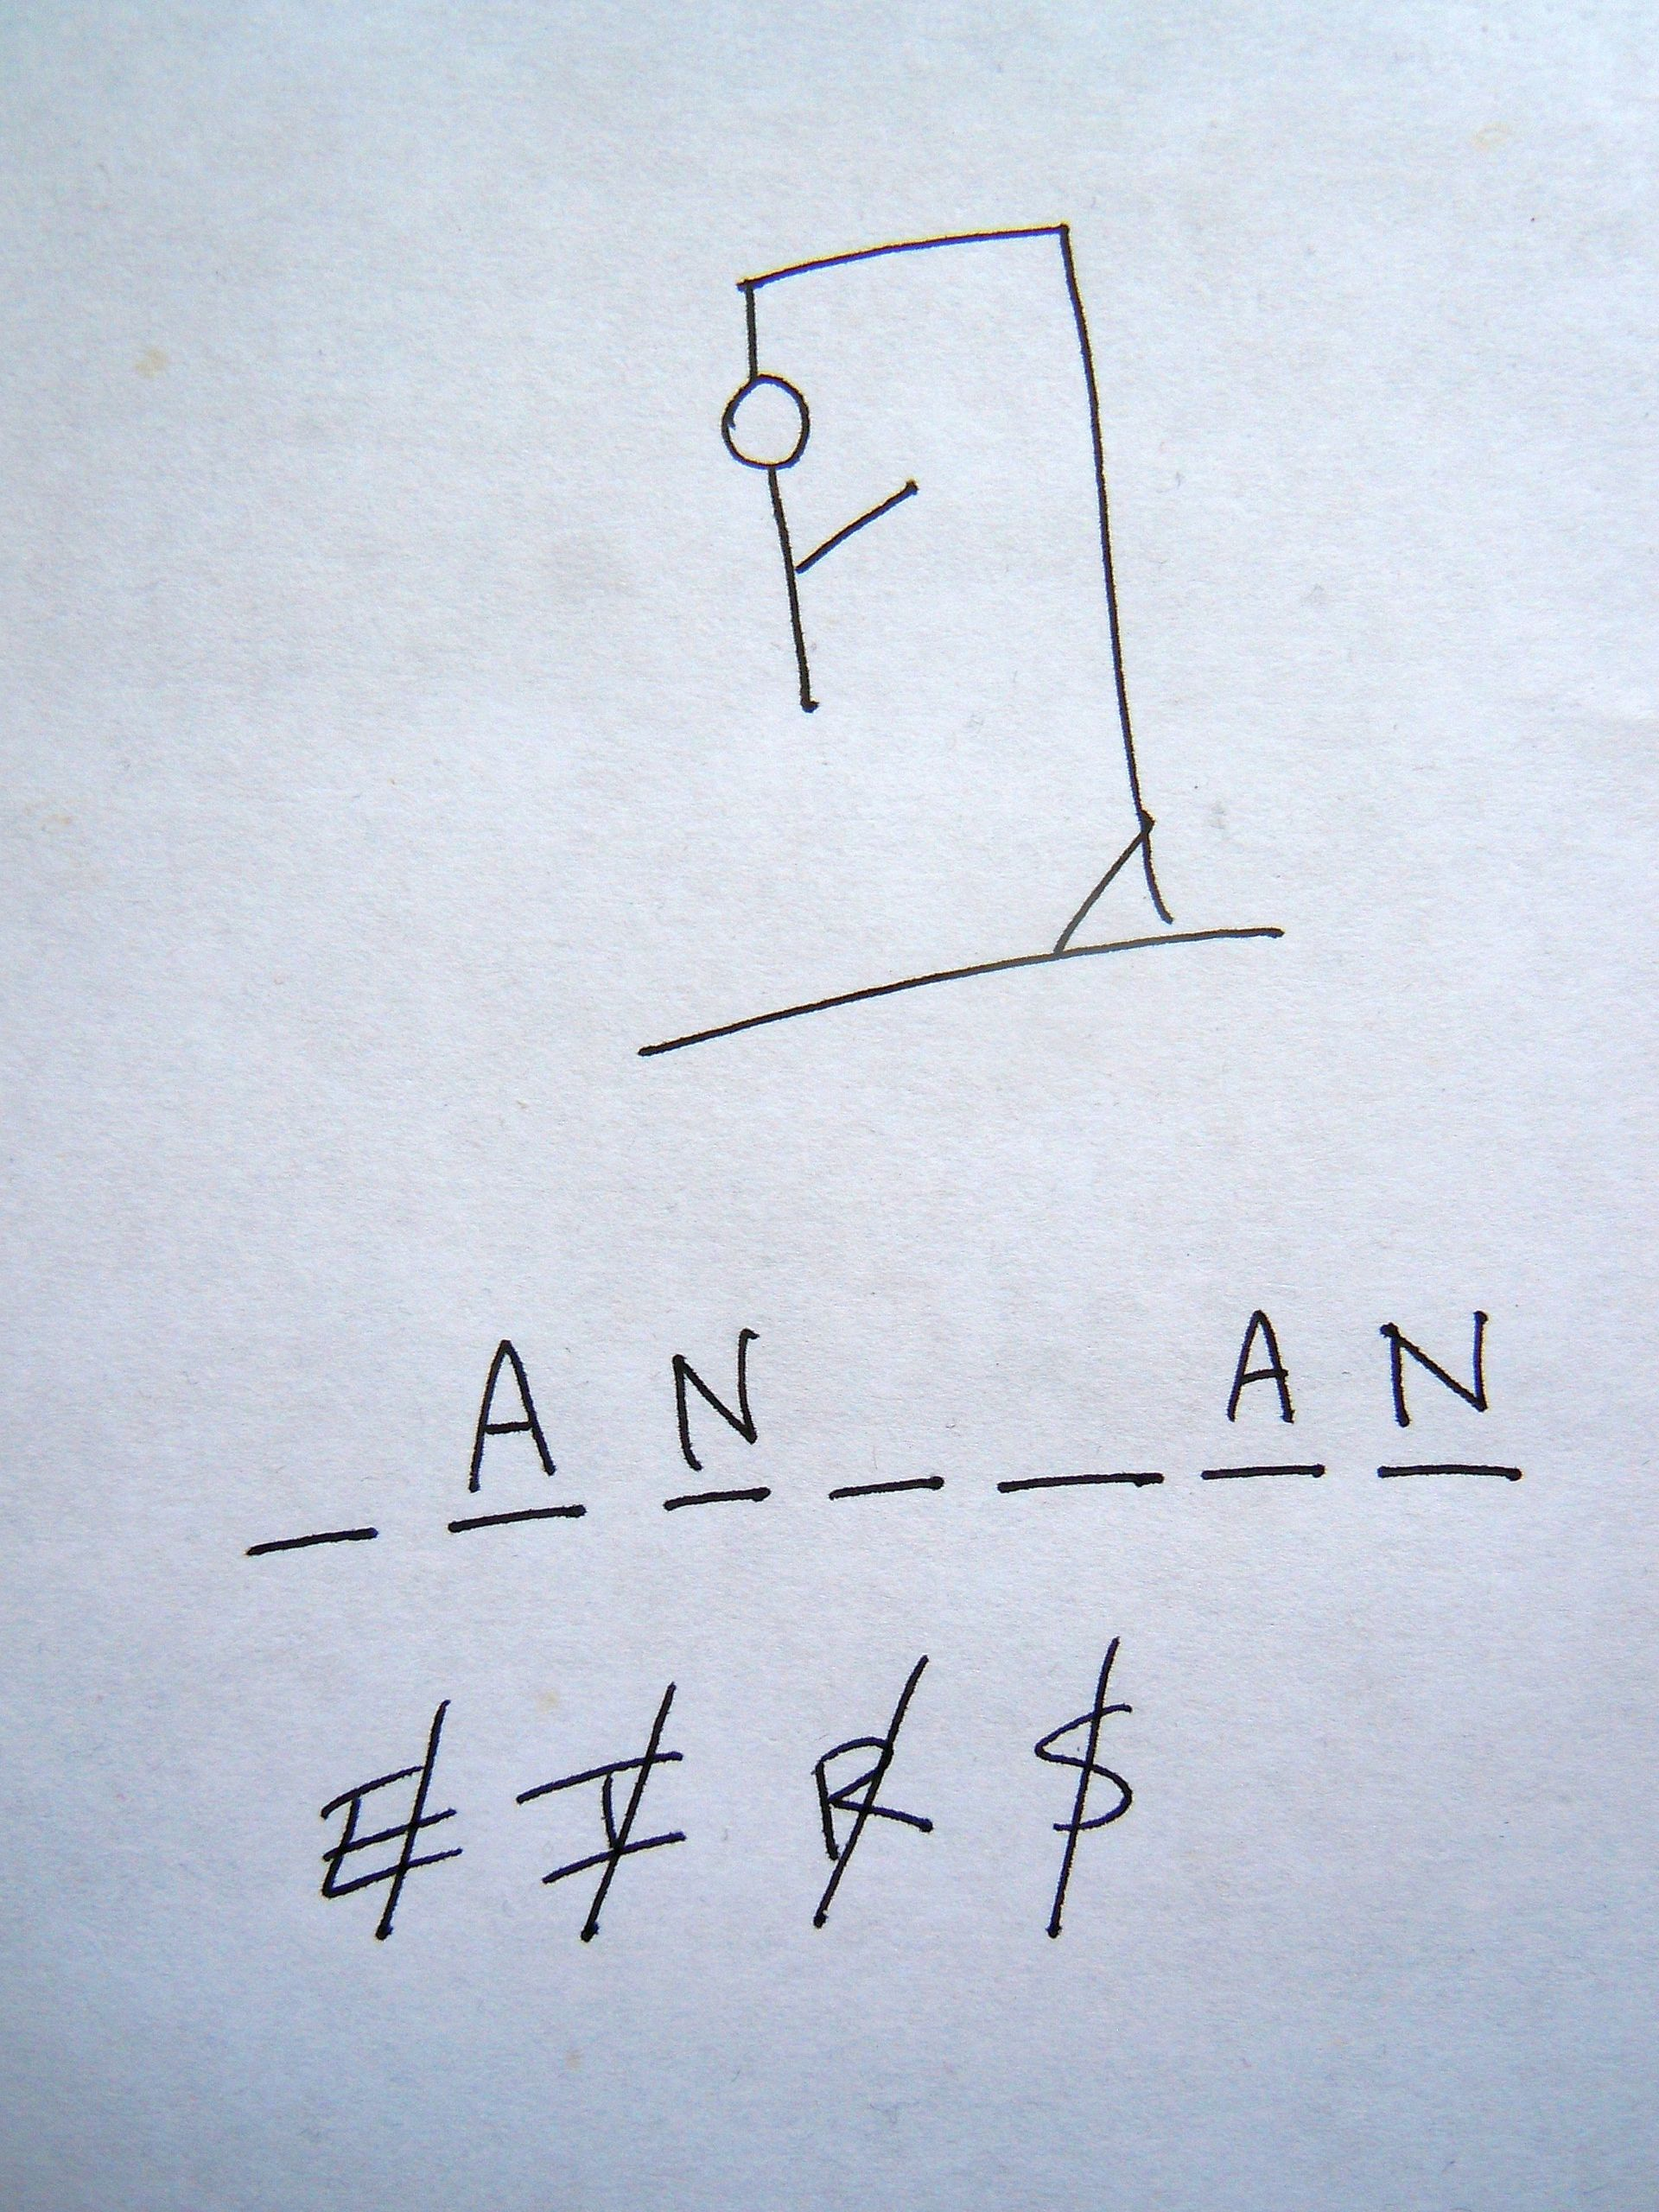
\includegraphics[width=0.8\textwidth]{hangman}
\label{fig:hangman}
\caption{Example hangman game}
\small{Taken from \url{https://upload.wikimedia.org/wikipedia/commons/thumb/f/f4/Hangman_game.jpg/1920px-Hangman_game.jpg}}
\end{figure}

\cprotect\sol{
<<<<<<< HEAD
\begin{python}
"""
This module implements the classic game hangman.

The goal of the game for the player is to guess a word the computer chose at
random by guessing individual letters. If one of the letters is part of the
chosen word, the computer tells the player the positions of all occurences.

The game consists of multiple rounds where the player can guess a letter
when prompted to do so.

If the guessed letter is in the word the computer chose, the game state is
updated and the player is presented with the positions of the letters they
guessed correctly.

If the guess was wrong, that means it is not part of the guess word, it is
added to the list of wrong guesses.

If the player guesses all letters before the number of wrong guesses
exceeds the number of allowed misses, they win. Otherwise the computer
wins.
"""
import random
import string


MAX_MISSES = 5
RULES = """
Hello! Let's play a game of hangman!
I already picked a word, and you now have to guess letters.
But be warned, if you guess wrong more than {} times, you lose!
""".format(MAX_MISSES)


def get_art(lvl=0, width=16):
    """
    Returns an array of lines of a hangman ascii art.

    The lines depend on the given level. The higher the level, the more
    of the man is displayed. The Art allows for 5 levels max.

    Args:
        lvl: the level to which the man is to be drawn
        width: what minimum width the drawing should have

    Returns:
        A list of strings, each string representing one line of the drawing,
        formatted to be at least `width` wide.
    """
    art_top = [" _______",
               "|      |"]
    if lvl < 5:
        art_mid = ["|", "|", "|", "|"]
        if lvl > 0:
            art_mid[0] = "|     (_) "
        if lvl > 1:
            art_mid[1] = "|     /|  "
        if lvl > 2:
            art_mid[1] = "|     /|\ "
        if lvl > 3:
            art_mid[2] = "|      |  "
            art_mid[3] = "|     /   "

        art_bot = ["|___________",
                   "/|       | |"]
    else:
        art_mid = [
            "|     (_)   ",
            "|     /|\   ",
            "|      |    ",
            "|     / \   "
        ]
        art_bot = ["|____    ___",
                   "/|   \   | |"]

    form = lambda s: "{0:{width}s}".format(s, width=width)

    art = [form(s) for s in art_top] +\
          [form(s) for s in art_mid] +\
          [form(s) for s in art_bot]
    
    return art


def read_words(file="words.txt"):
    """
    Reads a list of words from a file.

    There needs to be one word per line, for this to work properly.

    Args:
        file: the file to read from

    Returns:
        An array of all the words in the file
    """
    with open(file, "r") as f:
        return f.read().lower().splitlines()


def pick_word(words):
    """
    Chooses a random entry from the given list.

    Args:
        words: the list of words to pick a word from
    
    Returns:
        One word from the list `words`
    """
    return random.choice(words)


def get_guess():
    """
    Asks the user for an input letter until it is a valid letter.

    If the input is more than one character, or is not from the ascii
    alphabet (a-z), we ask the user again. We only deal with lowercase
    letters.

    Returns:
        The input guess from the user
    """
    guess = ""
    while (len(guess) != 1) or (not guess in string.ascii_lowercase):
        guess = input("Which letter is your next guess? ").lower()

    return guess


def print_game_state(turn, misses, guess_word, guesses):
    """
    Print the current state of the game.

    It displays a short header, and the ASCII art depending on how many
    misses there were already. It then displays the game state information:
    - How many misses we made
    - The current state of the guess word
    - The letters that were misses

    Args:
        turn: In which turn we are
        misses: how many misses are left
        guess_word: the current guess word
        guesses: the list of mistaken letters
    """
    # missed holds how many misses we made already
    missed = MAX_MISSES - misses

    # and empty line at the start
    space = ""
    header = "HANGMAN - THE GAME: Turn {}".format(turn)
    lines = [space] + [header] + get_art(missed)
    lines[2] += "MISSED: {} / {}".format(missed, MAX_MISSES)
    lines[3] += "GUESS THE WORD!"
    lines[4] += " ".join(guess_word)
    lines[6] += "Misses so far: " + ", ".join(guesses)
    
    # print the game state
    for line in lines:
        print(line)


def update_guess_word(word, guess_word, guess):
    """
    Updates the guess_word with the newly guessed letter.

    By iterating over the word and comparing each character, we can find
    all occurences of that letter and can replace the underscores in the
    guess word for each found occurence.

    E.g. if the word is 'hello' and the guess_word was ['_', 'e', '_', '_', '_']
    and the guess was 'l', the result will be ['_', 'e', 'l', 'l', '_']

    The function modifies the list in place.

    Args:
        word: the target word
        guess_word: the current state of the guess word
        guess: the guessed letter
    
    Returns:
        the updated state of the guess word. Though unnecessary, since lists
        are passed by reference and altered directly.
    """
    for i, letter in enumerate(word):
        if letter == guess:
            guess_word[i] = letter

    return guess_word


def print_guide():
    """Prints the rules of the game"""
    print(RULES)


def check_win(guess_word):
    """
    Returns True if the player has won.

    The player has won if there are no underscores left to guess.

    Args:
        guess_word: the current state of the guess word

    Returns:
        True in case of win, False otherwise.
    """
    return not "_" in guess_word


def game_end(won, word):
    """
    Prints a message depending on whether the player has won.
    
    Args:
        won: Boolean whether the player has won
        word: The target word
    """
    win_msg = "Congratulations!"
    lose_msg = "Oh no! Good luck next time! The word was {}"

    msg = win_msg if won else lose_msg.format(word)
    print(msg)


def init_guess_word(length):
    """
    Returns the initial guess word state.

    The guess word is initialised with underscores, one for each letter
    of the target word.

    Args:
        length: the length of the target word
    
    Returns:
        The initialised guess word, a list of `length` underscores
    """
    return ["_"] * length


def init():
    """
    Initialises our game world.

    Sets the default values for the game state variables, and then return
    them as a tuple. This includes to read the words from the file, picking
    a target word at random and initialising the guess word, as well as
    printing the guide to the game.

    Returns:
        The tuple that forms the game state.
    """
    turn = 0
    words = read_words()
    the_word = pick_word(words)
    guess_word = init_guess_word(len(the_word))
    misses = MAX_MISSES
    guesses = []

    print_guide()

    return turn, the_word, guess_word, misses, guesses


def game():
    """
    Runs the game loop.

    This function puts it all together to form the whole game. It initialises
    the game state values, and sets the default win state (false).
    It then loops until either the player has won, or the player missed all
    his allowed mistakes.
    In each loop we print the current state of the game, and get a new guessed
    letter. If it was a correct guess, we update the guess word and check
    whether the player has won, otherwise we decrement our allowed mistakes.

    Once the loop ends we print the game world one last time, and print
    the end of game message.
    """
    turn, word, guess_word, misses, guesses = init()
    won = False

    while not won and misses > 0:
        print_game_state(turn, misses, guess_word, guesses)
        guess = get_guess()

        if guess in word:
            guess_word = update_guess_word(word, guess_word, guess)
            won = check_win(guess_word)
        else:
            guesses += guess
            misses -= 1
        
        turn += 1

    print_game_state(turn, misses, guess_word, guesses)
    game_end(won, word)


# we can continue the game until the player quits
cont = "y"
while cont == "y":
    game() # play a game!
    # on a y or Y we continue
    cont = input("Do you want to play again? (y/n): ").lower()
\end{python}
=======
\pythonexternal{hangman.py}
>>>>>>> f02e5a0dc271881fab8d9e89529da082c88d8fae
}

\end{document}
